
\chapter{平台软件规划——连接确认(CC)}

 参考文件: Module Design of XX (Template).xlsx \cite{MDOT1};   
  
 \begin{enumerate}[label=\textbullet]
	\item  Introduce;
        \begin{enumerate}[label={}]
            \item \textcolor{red}{A brief description of the design module, which explains the functions that the modules needs to implement;}
        \end{enumerate}
	\item  Module Ports;
        \begin{enumerate}[label={}]
            \item \textcolor{red}{Don't need to write the specific ports, just write ``For more details about the modules ports, please refer to the related module interface files";}
        \end{enumerate}
	\item  Design Contents;
        \begin{enumerate}[label={}]
            \item \textcolor{red}{Before starting the design, the engineer should read the relevant information in ReadMe;}
        \end{enumerate}
\end{enumerate}

PP(Proximity Pilot)功能\cite{SAE}:PP 信号主要用于检测充电枪的物理状态,即充电插头的插
入深度和连接情况。PP 信号通过在插头和插座之间的物理连接来检测接近状态。作用:确认
充电枪是否插入到位。防止在插头未完全插入的情况下启动充电。确定充电电缆的额定电流
上限,以便限制通过充电线缆的最大电流,避免电缆过载。

CC(Connection Confirmation)功能\cite{GB18487_1}:CC 信号负责最终确认连接的整体安全性,并在
充电开始前完成所有必要的检查。它通常依赖于 CP 和 PP 信号提供的信息,以确定是否可以
安全地开始充电。作用:确认 PP 信号的接近检测状态,以及 CP 信号的通信和控制状态。在
确认连接安全、无误后,允许充电电流传输。如果在充电过程中发现任何异常情况,CC 信号
将触发充电中断。

充电规范GB-T 18487.1-2015\cite{GB18487_1}:
    \begin{enumerate}
        \item 对于充电模式3,可以ABC三种连接方式,单相供电最大电流不超过16 A;
        \item 对于充电模式3,三相供电时电流大于32 A应采样连接方式C;
    \end{enumerate}

本文档适用于充电设备在{\bf 充电模式3 连接方式B}工作状态下的使用规范。

\section{Introduce}
    连接确认模块(Connect comfirm),在SAE\_J1772中是接近检测(Proximity Detection)\cite{SAE}。 
    % 这两个信号的关系不一致: PP $\longrightarrow$ CP $\longrightarrow$ CC。
    PP信号主要用于检测充电枪的物理状态,即充电插头的插入深度和连接情况。PP信号通过在插头和插座之间的物理连接来检测接近状态。
    在交流充电系统中,CP(Control Pilot)信号和CC(Connection Confirmation)导线的电阻共同作用于确定最大充电电流。这是为了确保充电过程的安全性和兼容性。让我们分别来看CP和CC在这一过程中的角色及它们之间的关系。

 \begin{enumerate}
    \item  \textcolor{myred3}{确认充电枪是否插入到位},防止在插头未完全插入的情况下启动充电;
    \item  通过检测CC电阻值,车辆和充电桩可以确认充电枪是否正确插入,并\textcolor{myred3}{确定允许的最大充电电流}。
    \item 优先级机制:在实际应用中,CC 电阻的限流机制通常是最高优先级的。如果 CC
    电阻表明电缆只支持较小的电流,那么即使 CP 信号允许更大的电流,系统也会
    优先遵循 CC 导线的限流判断。
 \end{enumerate}

%  \begin{figure}[!htbp]
%     \centering
%     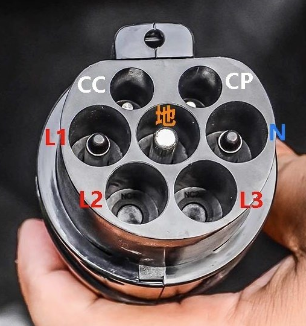
\includegraphics[width = 0.45\textwidth]{C3}
%     \caption{\href{https://www.chooseauto.com.cn/news/89436.shtml}{交流充电接口}}
%     \label{fig:C3}
% \end{figure}

\begin{figure}[!htbp]
    \centering
    \begin{subfigure}[b]{0.45\textwidth}
        \centering
        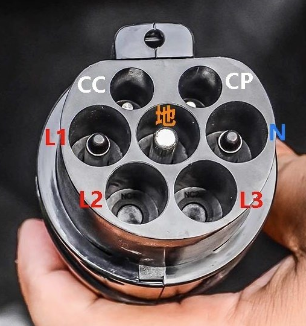
\includegraphics[width=0.65\textwidth]{C3} 
        \caption{交流充电接口}
        \label{fig:C3}
    \end{subfigure}
    \hspace*{-0.6cm}
    \begin{subfigure}[b]{0.45\textwidth}
        \centering
        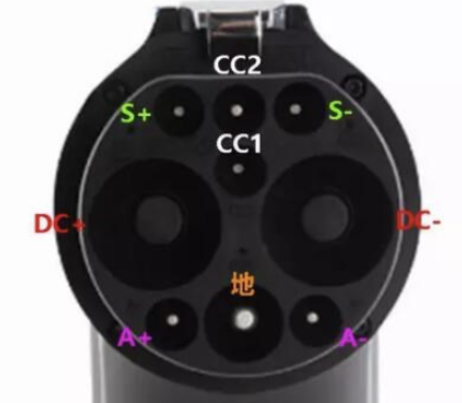
\includegraphics[width=0.8\textwidth]{C8} 
        \caption{直流充电接口}
        \label{fig:C8}
    \end{subfigure}
    \begin{subfigure}[b]{0.45\textwidth}
        \centering
        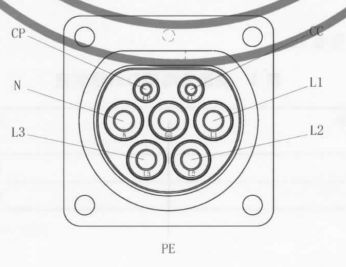
\includegraphics[width=0.8\textwidth]{C9} 
        \caption{交流充电接口\cite{GB20234_2}}
        \label{fig:C9}
    \end{subfigure}
    \hspace*{-0.6cm}
    \begin{subfigure}[b]{0.45\textwidth}
        \centering
        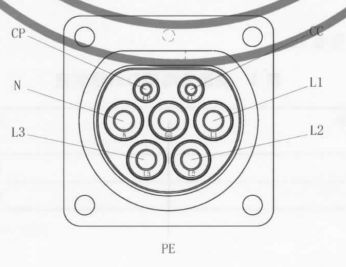
\includegraphics[width=0.8\textwidth]{C10} 
        \caption{直流充电接口\cite{GB20234_3}}
        \label{fig:C10}
    \end{subfigure}
    \caption{\href{https://www.chooseauto.com.cn/news/89436.shtml}{充电接口}}
    \label{fig:main}
\end{figure}



\begin{figure}[!htbp]
    \centering
    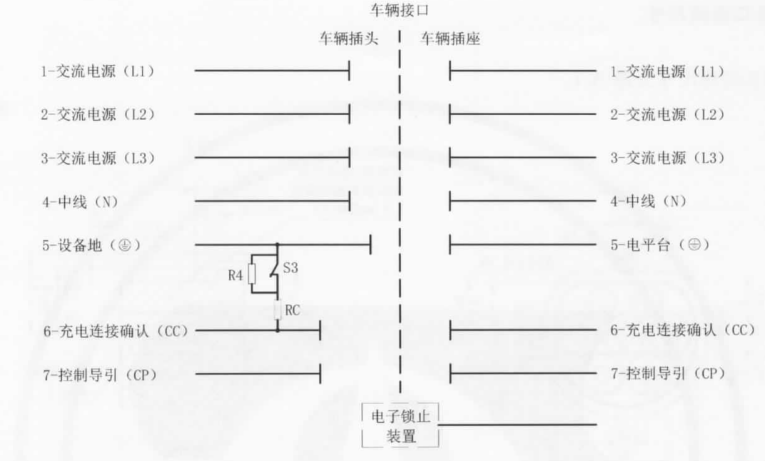
\includegraphics[width = 0.65\textwidth]{C5}
    \caption{车辆接口电气连接示意图}
    \label{fig:C5}
\end{figure}

\section{Modules Ports}


\section{Design Contents\_交流充电}

% (1) 车辆控制装置测量检测点 2 有无 12 V CP 信号。如有
% 则标志着车辆插头与车辆插座已连接,控制导引电
% 路激活进入工作状态;如无,则控制导引电路处于
% 待机状态。%[8]。

% (2) 车辆控制装置通过测量检测点 3 与
% PE 之间的电阻值来判断车辆插头与车辆插座是否
% 完全连接。半连接时,S3 断开,检测点 3 与 PE 之
% 间的电阻为 RC+R4;完全连接时,S3 处于闭合状
% 态,检测点 3 与 PE 之间的电阻值为 RC。

% (3) 供电控制装置通过测量检测点 1 的电压判断 R3 是否接
% 入,如 R3 接入则延时一定时间,将 S1 切换至 PWM输出状态。

% (4) 车辆检测装置通过测量检测点 2 的
% PWM 信号,判断充电装置是否已经完全连接。如
% 完全连接,则闭合开关 S2,车辆进入准备就绪状态。

% (5) 供电控制装置通过进一步测量检测点 1 的电压
% 判断车辆是否进入准备就绪状态,如已进入就绪状
% 态,则闭合 K1、K2,交流供电回路导通。%[11]。

% (6) 车辆控制装置通过测量检测点 2 的 PWM 信号占空比
% 确认供电设备的最大供电能力,并以此确定车载充
% 电机的输出电流,启动充电过程。%[9]。


\begin{figure}[!htbp]
    \centering
    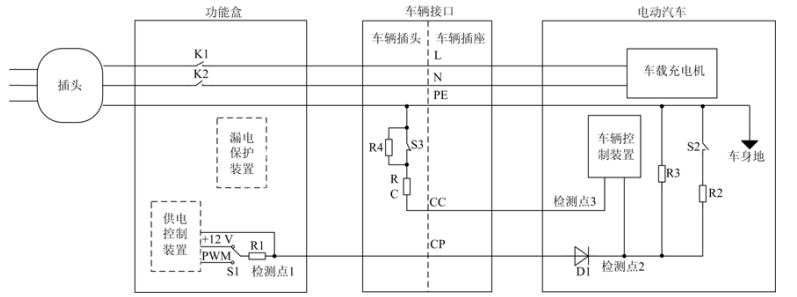
\includegraphics[width = 0.82\textwidth]{C4}
    \caption{交流充电模式2连接方式B\cite{GB18487_1}}
    \label{fig:C4}
\end{figure}



\subsection{计算流程}
\subsubsection*{电流因子}
        计算电流的原始采样值:
            \begin{equation}
                \mathrm{Raw\_CC\_Voltage} = \mathrm{CC\_Voltage\_Factor} \times  \mathrm{ADC\_CC\_Voltage}
                \label{eq:CC1}
            \end{equation}

    \subsubsection*{一阶滤波}
        采样频率100 Hz,无延时;一阶传递函数表示如下:
            \begin{equation}
                G(s) = \frac{\omega_c}{s+\omega_c}
                \label{eq:CC2}
            \end{equation}
        或者:
            \begin{equation}
                G(s) = \frac{1}{T_cs+1}
                \label{eq:CC3}
            \end{equation}
        其中,$\omega_c$表示截止频率,$T_c$表示时间常数。离散化,后向差分,令$s = \frac{1-z^{-1}}{T_s}$, $T_s$表示采样周期。
        可以得到差分方程:
            \begin{equation}
                y(k) = \frac{\omega_cT_s}{1+\omega_cT_s}x(k)+\frac{1}{1+\omega_cT_s}y(k-1)
            \end{equation}
        令$a = \frac{\omega_cT_s}{1+\omega_cT_s}$, $1-a = \frac{1}{1+\omega_cT_s} $:
            \begin{equation}
                y(k) = ax(k)+(1-a)y(k-1)
                \label{eq:CC4}
            \end{equation}
        \textcolor{red}{CC\_Current滤波:}
            \begin{enumerate}[label={}]
                \item $y = \mathrm{Samp\_CC\_Voltage} $;
                \item $x = \mathrm{Raw\_CC\_Voltage} $;
                \item $a = \mathrm{CC\_Current\_FilterFactor}$
            \end{enumerate}
        系数$a$决定了滤波器的带宽:
            \begin{equation}
                \begin{cases}
                    \text{当 $a$ 较小时,滤波平稳,灵敏度低}\\
                    \text{当 $a$ 较大时,滤波毛刺大,灵敏度高}
                \end{cases}
            \end{equation}

        \subsubsection*{陷波滤波器}
            1.连续时间传递函数:
                \begin{equation}
                    N(s) = \frac{s^2 + 2\cdot g_\mathrm{min} \cdot \mathrm{freq} \cdot \mathrm{damp}\cdot s + \mathrm{freq}^2}{s^2 + 2\cdot \mathrm{freq} \cdot \mathrm{damp} \cdot s + \mathrm{freq}^2}
                    \label{eq:Cxb}
                \end{equation}
          
            2. 令$s = \frac{1-z^{-1}}{T_s}$, $T_s$表示采样周期: 
                \begin{equation}
                    N(z) = \frac{1 - \left(2 + 2 \cdot \text{damp} \cdot \text{freq} \cdot T_s\right)z^{-1} + \left(1 - 2 \cdot \text{damp} \cdot \text{freq} \cdot T_s + \text{freq}^2 \cdot T_s^2\right)z^{-2}}{1 - \left(2 + 2 \cdot g_{\text{min}} \cdot \text{damp} \cdot \text{freq} \cdot T_s\right)z^{-1} + \left(1 - 2 \cdot g_{\text{min}} \cdot \text{damp} \cdot \text{freq} \cdot T_s + \text{freq}^2 \cdot T_s^2\right)z^{-2}}
                \end{equation}

            3. 差分方程形式:
            \begin{equation}
                y(k) = b_0 \cdot x(k) + b_1 \cdot x(k-1) + b_2 \cdot x(k-2) - a_1 \cdot y(k-1) - a_2 \cdot y(k-2)
            \end{equation}
            其中:
                \begin{equation}
                    \begin{aligned}
                        a_1 &= 2 + 2 \cdot \text{damp} \cdot \text{freq} \cdot T_s \\
                        a_2 &= 1 - 2 \cdot \text{damp} \cdot \text{freq} \cdot T_s + \text{freq}^2 \cdot T_s^2 \\
                        b_0 &= 1 \\
                        b_1 &= 2 + 2 \cdot g_{\text{min}} \cdot \text{damp} \cdot \text{freq} \cdot T_s \\
                        b_2 &= 1 - 2 \cdot g_{\text{min}} \cdot \text{damp} \cdot \text{freq} \cdot T_s + \text{freq}^2 \cdot T_s^2.
                        \end{aligned}
                \end{equation}
            举例:
            \begin{equation}
                \begin{aligned}
                    &\text{damp} = 30 \\
                    &\text{freq} = 50 \cdot  2\pi \\
                    &g_{\text{min}} =  0.01\\
                    &T_s = 0.001.
                    \end{aligned}
            \end{equation}
        
        \subsubsection*{双线性变换陷波滤波器}
            令 $s = \frac{2}{T_s}\frac{1-z^{-1}}{1+z^{-1}}$, 带入连续模型(\ref{eq:Cxb}):
        \begin{lstlisting}[language = matlab]
            % 定义s变量
            s = tf('s');
            % 例如:定义一个二阶系统传递函数
            freq = 50*2*pi;       % 频率
            damp = 3;             
            gmin = 0.01;
            H_s = (s^2 + 2*damp*freq*gmin*s + freq^2) / (s^2 + 2*damp*freq*s + freq^2)
            Ts = 0.001;  % 采样时间
            H_z = c2d(H_s, Ts, 'tustin')
        \end{lstlisting}
        

        \subsubsection*{RC电阻测量}
            \begin{figure}[H]
                \centering
                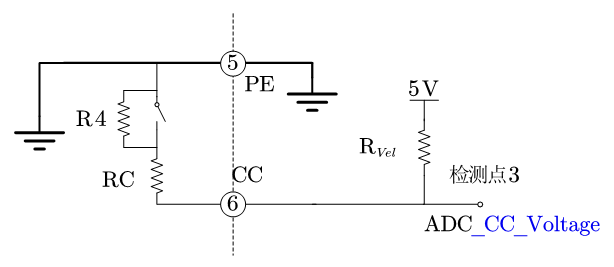
\includegraphics[width = 0.82\textwidth]{CC检测电路}
                \caption{CC电压检测}
                \label{fig:C13}
            \end{figure}


        \begin{table}[!htbp]
            \renewcommand{\arraystretch}{1.3}
            \centering
            \caption{车辆连接状态及RC阻值\cite{GB18487_1}}
            \begin{tabular}{ccccc}   
                 \toprule
                 状态  & RC  & R4 & S3 & 连接状态及额定电流\\    
                 \midrule
                 状态A  & -  & - & - &  车辆未连接 \\
                 状态C  & 1.5 k$\Omega$  & - & 闭合 &  车辆接口完全连接,最大充电电流10 A \\
                 状态D  & 680 $\Omega$  & - &  闭合 &  车辆接口完全连接,最大充电电流16 A  \\
                 状态E  & 220 $\Omega$ & - &   闭合 &  车辆接口完全连接,最大充电电流32 A  \\
                 状态F  & 100 $\Omega$ & - &   闭合 &  车辆接口完全连接,最大充电电流63 A  \\
                 状态B  & \multicolumn{2}{c}{Rc+R4 = 3.3$\thicksim$ 3.52 k$\Omega$} & 断开 &车辆接口处于半连接状态\\
                 \bottomrule
            \end{tabular}
            \label{tab:RC1}
       \end{table}
       定义车辆内部的检测电压为$V_{Vel}$, 预设电阻为$R_{Vel}$, 检测点的电压$V_{cc}$为:
            \begin{equation}
                V_{cc} = \frac{Rc}{R_{Velcc}+Rc} V_{Velcc}
            \end{equation}

       \begin{example}
         假设充电机的检测电压为$V_{Vel} = 5 \mathrm{V}$, 预设电阻为 $R_{Vel} = 500 \Omega$。
            \begin{table}[H]
                \renewcommand{\arraystretch}{1.3}
                \centering
                \caption{车辆连接状态及RC阻值}
                \begin{tabular}{ccccc}   
                    \toprule
                    状态  & RC  & R4 & $V_{cc}$ & 连接状态及额定电流\\    
                    \midrule
                    状态A  & -  & - & 5 V &   \\
                    状态C  & 1.5 k$\Omega$  & - & 3.75 V &  10 A \\
                    状态D  & 680 $\Omega$  & - &  2.88 V &  16 A  \\
                    状态E  & 220 $\Omega$ & - &   1.53 V &  32 A  \\
                    状态F  & 100 $\Omega$ & - &   0.88 V &  63 A  \\
                    状态B  & \multicolumn{2}{c}{3.3$\thicksim$ 3.52 k$\Omega$} & 4.34 V &车辆接口处于半连接状态\\
                    \bottomrule
                \end{tabular}
                \label{tab:RC2}
            \end{table}

            状态与检测电压之间的关系:
            \begin{table}[H]
                \renewcommand{\arraystretch}{1.3}
                \centering
                \caption{ 状态与检测电压之间的关系}
                \begin{tabular}{cccc}   
                    \toprule
                    CCM\_CC\_ACStatus  &  CC\_Voltage\_Limit$i$  & 状态描述 & CCM\_CC\_MaxACCurent(0.1 A)\\    
                    \midrule
                    0  &  5 V    &   AC\_DisConnect  & 0 \\
                    1  &  3.75 V &    ChargConnectState\_AC10A & 100\\
                    2  &  2.88 V &   ChargConnectState\_AC16A & 160  \\
                    3  &  1.53 V &   ChargConnectState\_AC32A & 320 \\
                    4  &  0.88 V &   ChargConnectState\_AC63A & 630 \\
                    5  &  4.34 V &    AC\_SemiConnect          &    0\\
                    6  &  其他电压值 & AC\_ErrConnect          & 0\\
                    \bottomrule
                \end{tabular}
                \label{tab:RC3}
            \end{table}
            根据不同Rc电阻采样的电压值判断连接状态,采样点为检测点3的电压SAMP\_CC\_Voltage, 更加采样电路预设6个电压等级CC\_Voltage\_Limit$i$($i=0,1,2,3,4,5$):
                \begin{enumerate}
                    \item SAMP\_CC\_Voltage == CC\_Voltage\_Limit0 $\pm$ $ \delta $: 交流充电未连接;
                    \item SAMP\_CC\_Voltage == CC\_Voltage\_Limit1 $\pm$ $ \delta $: 交流充电10 A;
                    \item SAMP\_CC\_Voltage == CC\_Voltage\_Limit2 $\pm$ $ \delta $: 交流充电16 A;
                    \item SAMP\_CC\_Voltage == CC\_Voltage\_Limit3 $\pm$ $ \delta $: 交流充电32 A;
                    \item SAMP\_CC\_Voltage == CC\_Voltage\_Limit4 $\pm$ $ \delta $: 交流充电63 A;
                    \item SAMP\_CC\_Voltage == CC\_Voltage\_Limit5 $\pm$ $ \delta $: 交流充电半连接;
                    \item SAMP\_CC\_Voltage != CC\_Voltage\_Limit$i$ $\pm$ $ \delta $: 交流充电连接错误;
                \end{enumerate} 
       \end{example}

    
   
        






\subsection{交流充电控制流程}
    \begin{table}[H]
        \begin{minipage}[p]{0.46\textwidth} 
            \centering 
            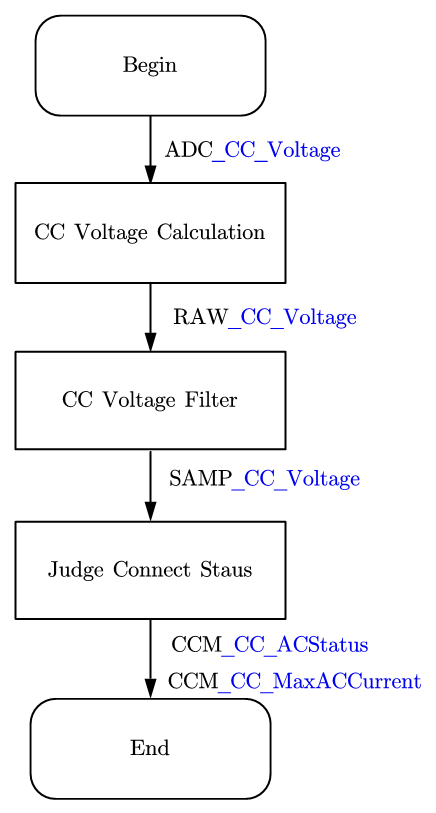
\includegraphics[width=60mm]{CC流程图} 
        \end{minipage}
            \begin{minipage}[p]{0.46\textwidth}
            \centering
            \renewcommand{\arraystretch}{1.3}
                \begin{tabular}{|c|c|c|c|}
                    \specialrule{0.2em}{0pt}{0pt} 
                    \textbf{Input Port} & Range & Data Type & Unit \\
                    \hline
                    ADC\_CC\_Voltage& -  & Uint16 & -  \\
                    \hline
                    &  & &\\
                    \specialrule{0.2em}{0pt}{0pt} 
                    \textbf{Output Port}    &   \multicolumn{3}{c|}{}\\
                    \hline
                      CCM\_CC\_ACMaxCurrent                      &  & Uint16 &  0.1 A\\
                    \hline
                      CCM\_CC\_ACStatus                      &  & Uint8  & \\
                    \hline
                    &  & &\\
                    \specialrule{0.2em}{0pt}{0pt} 
                    \textbf{Parameter Port}    &   \multicolumn{3}{c|}{}\\
                    \hline
                        CC\_Voltage\_Factor                      &  & Folat32 & \\
                        \hline
                        CC\_Voltage\_FilterFactor                & 0$\sim$1 & Folat16 & \\
                        \hline
                        CC\_Voltage\_Limit$i$(i=0$\sim$5 )       & 0$\sim$5 & Folat32 & 1 V\\
                    \specialrule{0.2em}{0pt}{0pt} 
                \end{tabular} 
            \end{minipage}
        \caption{\textcolor{red}{(a)CC流程图. (b)输入输出接口.}} 
        \label{tab:figtab1} 
    \end{table}

    % \begin{minipage}{0.45\textwidth}
    %     \centering
    %     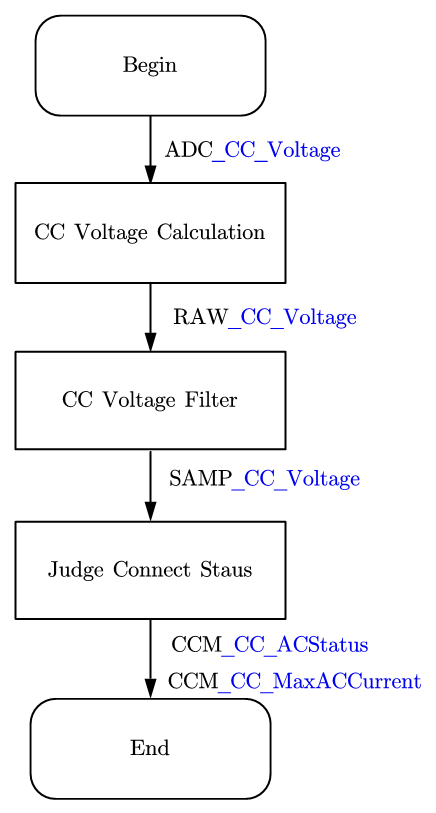
\includegraphics[width=0.9\textwidth]{CC流程图}
    %     % \caption{CC流程图}
    %     % \label{fig:CClc}    
    % \end{minipage}
    % \hfill
    % \begin{minipage}{0.45\textwidth}
    %     \renewcommand{\arraystretch}{1.3}
    %     % \captionof{table}{国内外电动主要传导式充电系统标准}
    %     \begin{tabular}{c|c|c|c|c|c|c}
    %         \specialrule{0.2em}{0pt}{0pt} 
    %         \multicolumn{2}{c|}{类别} & 2 & 3 & 4& 5 & 6\\
    %         \hline
    %         \multicolumn{2}{c|}{类别} & 2 & 3 & 4& 5 & 6\\
    %         \hline
    %         \multirow{3}{*}{合并的行} & 1 &2 &3&4&5&6\\
    %                                 & 1 &2 &3&4&5&6\\
    %                                 & 1 &2 &3&4&5&6\\
    %         \hline
    %         \multicolumn{2}{c|}{类别} & 2 & 3 & 4& 5 & 6\\
    %         \specialrule{0.2em}{0pt}{0pt} 
    %     \end{tabular} 
    % \end{minipage}


    \begin{algorithm}[H] 
        % \SetAlgoLined
        \caption{连接确认(Connection Confirmation)——交流充电} 
        \label{alg3} 
        \makebox[1\textwidth][c]{ % 设置宽度为文本宽度并居中
        \begin{minipage}{0.91\textwidth} % 设置算法宽度为 80% 文本宽度
        \renewcommand{\baselinestretch}{1.5} % 设置行距为 1.5 倍
        \selectfont
        \begin{algorithmic}[1] % [1] 表示显示行号
            \REQUIRE ADC\_CC\_Current, CC\_Current\_Limit$i$($i=0,1,2,3,4,5$);
            \ENSURE CCM\_CC\_Status, CCM\_CC\_MaxACCurent;
            \STATE Begin
            \STATE 获取CC电流AD采样值:ADC\_CC\_Current;
            \STATE 1)计算CC原始采样电流:Raw\_CC\_Current,根据公式(\ref{eq:CC1});
            \STATE 2)计算CC滤波采样电流: Samp\_CC\_Current,根据公式(\ref{eq:CC4});
            \STATE 3)判断连接状态,根据表(\ref{tab:RC2});
            \IF{Samp\_CC\_Current == CC\_Current\_Limit$i$ $\pm \, 0.1$ V } 
                \STATE CCM\_CC\_ACStatus = $i$
            \ELSIF{Samp\_CC\_Current != CC\_Current\_Limit$i$}
                \STATE CCM\_CC\_ACStatus = 6 连接异常
            \ENDIF
            \STATE End 
        \end{algorithmic} 
        \end{minipage}
        }
    \end{algorithm}





%%%%%%%%%%%%%%%%%%%%%%%%%%%%%%%%%%%%%%%%%%%%%%%%%%%%%%%%%%%%%%%%%%%%%%%% 交流放电 %%%%%%%%%%%%%%%%%%%%%%%%%%%%%%%%%%%%%%%%%%%%%%%%%


\clearpage
    \section{Design Contents\_交流放电}
    \textcolor{myred}{\textbf{放电模式1.1 交流V2L}}\cite{GB18487_4}\\
     交流V2L放电使用传导连接组件连接用电负荷,能量传输过程中采用单相或三相放电,放电车辆总放电电流单相不超过32A,三相不超过63A。传导连接组件如有多路输出,每路输出宜分别具备过流保护,如图(\ref{fig:V2L})。
        \begin{figure}[H]
            \centering
            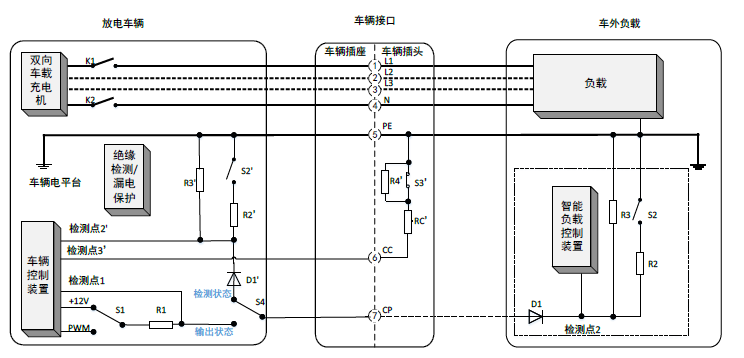
\includegraphics[width = 0.9\textwidth]{V2L控制引导}
            \caption{V2L 模式控制导引电路原理图}
            \label{fig:V2L}
        \end{figure}
    \textcolor{myred}{\textbf{放电模式1.2 交流V2V}}\cite{GB18487_4}\\
    模式1.2用于放电车辆对电动汽车交流放电,能量传输过程中采用单相或三相电,单相放电不超过32A,三相放电不超过63A。
    放电引导电路如图(\ref{fig:V2V}),提供放电控制功能。放电接口应符合GB/T20234.2的规定\cite{GB18487_2}。%从放电车辆到充电车辆宜提供保护接地导体,且具备绝缘监测功能。
        \begin{figure}[H]
            \centering
            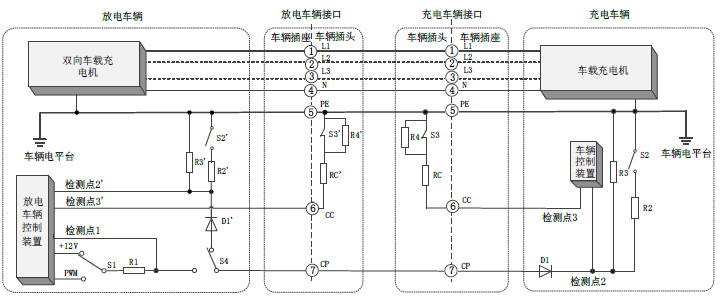
\includegraphics[width = 0.9\textwidth]{V2V控制引导}
            \caption{V2V 的控制导引电路原理图}
            \label{fig:V2V}
        \end{figure}

        \begin{lstlisting}[language = matlab]
            Vvel=5;
            Rvel =800;
            
            G2V_Rc= [1500,680,220,100,3300,3500];   %放电RC电阻计算
                V1 = G2V_Rc(1)/(G2V_Rc(1)+Rvel) * Vvel;
                V2 = G2V_Rc(2)/(G2V_Rc(2)+Rvel) * Vvel;
                V3 = G2V_Rc(3)/(G2V_Rc(3)+Rvel) * Vvel;
                V4 = G2V_Rc(4)/(G2V_Rc(4)+Rvel) * Vvel;
                V51 = G2V_Rc(5)/(G2V_Rc(5)+Rvel) * Vvel;
                V52 = G2V_Rc(6)/(G2V_Rc(6)+Rvel) * Vvel;
                V_G2V = [V1, V2, V3,V4,V51,V52]'
                      
            V2L_Rc= [2700,2000,1000,470,3300,3500]; %放电RC电阻计算
                V11 = V2L_Rc(1)/(V2L_Rc(1)+Rvel) * Vvel;
                V22 = V2L_Rc(2)/(V2L_Rc(2)+Rvel) * Vvel;
                V33 = V2L_Rc(3)/(V2L_Rc(3)+Rvel) * Vvel;
                V44 = V2L_Rc(4)/(V2L_Rc(4)+Rvel) * Vvel;
                V551 = V2L_Rc(5)/(V2L_Rc(5)+Rvel) * Vvel;
                V552 = V2L_Rc(6)/(V2L_Rc(6)+Rvel) * Vvel;
                V_V2L = [V11, V22, V33,V44,V551,V552]'
            
            Vall = sort([V_G2V;V_V2L])
        \end{lstlisting}


